%-- Template based off http://www.latextemplates.com/template/structured-general-purpose-assignment.

%%%%%%%%%%%%%%%%%%%%%%%%%%%%%%%%%%%%%%%%%
% Structured General Purpose Assignment
% LaTeX Template
%
% This template has been downloaded from:
% http://www.latextemplates.com
%
% Original author:
% Ted Pavlic (http://www.tedpavlic.com)
%
% Note:
% The \lipsum[#] commands throughout this template generate dummy text
% to fill the template out. These commands should all be removed when 
% writing assignment content.
%
%%%%%%%%%%%%%%%%%%%%%%%%%%%%%%%%%%%%%%%%%

%----------------------------------------------------------------------------------------
%	PACKAGES AND OTHER DOCUMENT CONFIGURATIONS
%----------------------------------------------------------------------------------------

\documentclass{article}

\usepackage{fancyhdr} % Required for custom headers
\usepackage{lastpage} % Required to determine the last page for the footer
\usepackage{extramarks} % Required for headers and footers
\usepackage{graphicx} % Required for including pictures
\usepackage{biblatex}
\usepackage{caption}
\usepackage{float}
\usepackage[none]{hyphenat}


\bibliography{main.bib}
\graphicspath{ {images/} }

% Margins
\topmargin=-0.45in
\evensidemargin=0in
\oddsidemargin=0in
\textwidth=6.5in
\textheight=9.0in
\headsep=0.25in 

\linespread{1.1} % Line spacing

% Set up the header and footer
\pagestyle{fancy}
\lhead{\hmwkTitle} % Top left header
\chead{\hmwkShortCode} % Top center header
\rhead{\hmwkAuthorName} % Top right header
\lfoot{\lastxmark} % Bottom left footer
\cfoot{} % Bottom center footer
\rfoot{Page\ \thepage\ of\ \pageref{LastPage}} % Bottom right footer
\renewcommand\headrulewidth{0.4pt} % Size of the header rule
\renewcommand\footrulewidth{0.4pt} % Size of the footer rule

\setlength\parindent{0pt} % Removes all indentation from paragraphs

%----------------------------------------------------------------------------------------
%	DOCUMENT STRUCTURE COMMANDS
%	Skip this unless you know what you're doing
%----------------------------------------------------------------------------------------

% Header and footer for when a page split occurs within a problem environment
\newcommand{\enterProblemHeader}[1]{
\nobreak\extramarks{#1}{#1 continued on next page\ldots}\nobreak
\nobreak\extramarks{#1 (continued)}{#1 continued on next page\ldots}\nobreak
}

% Header and footer for when a page split occurs between problem environments
\newcommand{\exitProblemHeader}[1]{
\nobreak\extramarks{#1 (continued)}{#1 continued on next page\ldots}\nobreak
\nobreak\extramarks{#1}{}\nobreak
}

\setcounter{secnumdepth}{0} % Removes default section numbers
\newcounter{homeworkProblemCounter} % Creates a counter to keep track of the number of problems

\newcommand{\homeworkProblemName}{}
\newenvironment{homeworkProblem}[1][Problem \arabic{homeworkProblemCounter}]{ % Makes a new environment called homeworkProblem which takes 1 argument (custom name) but the default is "Problem #"
\stepcounter{homeworkProblemCounter} % Increase counter for number of problems
\renewcommand{\homeworkProblemName}{#1} % Assign \homeworkProblemName the name of the problem
\section{\homeworkProblemName} % Make a section in the document with the custom problem count
\enterProblemHeader{\homeworkProblemName} % Header and footer within the environment
}{
\exitProblemHeader{\homeworkProblemName} % Header and footer after the environment
}

\newcommand{\problemAnswer}[1]{ % Defines the problem answer command with the content as the only argument
\noindent\framebox[\columnwidth][c]{\begin{minipage}{0.98\columnwidth}#1\end{minipage}} % Makes the box around the problem answer and puts the content inside
}

\newcommand{\homeworkSectionName}{}
\newenvironment{homeworkSection}[1]{ % New environment for sections within homework problems, takes 1 argument - the name of the section
\renewcommand{\homeworkSectionName}{#1} % Assign \homeworkSectionName to the name of the section from the environment argument
\subsection{\homeworkSectionName} % Make a subsection with the custom name of the subsection
\enterProblemHeader{\homeworkProblemName\ [\homeworkSectionName]} % Header and footer within the environment
}{
\enterProblemHeader{\homeworkProblemName} % Header and footer after the environment
}
   
%----------------------------------------------------------------------------------------
%	NAME AND CLASS SECTION
%----------------------------------------------------------------------------------------

\newcommand{\hmwkTitle}{Enhancing the CS-Alumni Application} % Assignment title
\newcommand{\hmwkDueDate}{Monday,\ Decemeber\ 8,\ 2014} % Due date
\newcommand{\hmwkShortCode}{SE31520}
\newcommand{\hmwkClass}{Developing Internet-Based Applications} % Course/class
\newcommand{\hmwkClassTime}{4pm} % Class/lecture time
\newcommand{\hmwkAuthorName}{Thomas Mark Rosier (THR2)} % Your name
\newcommand{\hmwkStudentId}{110113188} % Student ID

%----------------------------------------------------------------------------------------
%	TITLE PAGE
%----------------------------------------------------------------------------------------

\title{
\vspace{2in}
\textmd{\textbf{\hmwkShortCode\\ \hmwkClass}}\\
\normalsize
\vspace{0.1in}
\textbf{\hmwkTitle}\\
\vspace{0.1in}
\small{Submission\ Due\ \hmwkClassTime\ \hmwkDueDate}\\
\vspace{3in}
}

\author{
\textbf{\hmwkAuthorName}\\
\hmwkStudentId
}
\date{} % Insert date here if you want it to appear below your name

%----------------------------------------------------------------------------------------

\begin{document}

\maketitle

%----------------------------------------------------------------------------------------
%	TABLE OF CONTENTS
%----------------------------------------------------------------------------------------

%\setcounter{tocdepth}{1} % Uncomment this line if you don't want subsections listed in the ToC

\newpage
\tableofcontents
\newpage


\nocite{bara:2013:online}
\nocite{saa:2013:online}

%-- Document Summary.
\section{Document Summary}

\iffalse
 _________    ________      ________      ________     
|\___   ___\ |\   __  \    |\   ___ \    |\   __  \    
\|___ \  \_| \ \  \|\  \   \ \  \_|\ \   \ \  \|\  \   
     \ \  \   \ \  \\\  \   \ \  \ \\ \   \ \  \\\  \  
      \ \  \   \ \  \\\  \   \ \  \_\\ \   \ \  \\\  \ 
       \ \__\   \ \_______\   \ \_______\   \ \_______\
        \|__|    \|_______|    \|_______|    \|_______|                                               
\fi   

%-- Application Design.
\section{Application Design}

\subsection{CS-Alumni Chrome Browser Extension}

\subsubsection{Rational}

My rational behind deciding to developing a browser extension for this project, was that they have been a technology that I have been following for a while and I have not seen them used that regularly for small little applications that interface with a bigger application.\\
\\
Another reason for my choice to develop a browser extension was that I wanted to learn about implementing some of the more advanced features within the Chrome SDK for example the use of 'Background Pages' which are used to keep a task running in the background while the extension is closed.\\
\\
One of the newer features within the Chrome SDK had also caught my attention in the weeks before starting this assignment was the use of Chrome desktop notifications where you can create a notification within your application that will be displayed to the end user via the Chrome UI's notification draw.\\
\\
I wanted to see if it was possible to encapsulate some of the key management features of the CS-Alumni application into an attractive and well presented browser extension that also notified the user of any new broadcasts that had been made.\\
\\
Why did I choose to develop a Chrome extension over a Firefox, Safari or Internet Explorer, the main reason was due to Chris Loftus's preference of Chrome over the other browsers. In addition to that I felt that due to developing for Chrome also meant that the code will work without modification in Opera this a bonus in the real world as it means we can support a greater population of users without investing more money into development.\\
\\
I also feel that Chrome has a much nicer development environment for developing browser extensions over its competitors, along with having some newer and more unique features that allow the Chrome based extension to stand out.\\
\\
If this was a real world product it would not take that much resources to port the extension to work on Firefox and Safari aswell but this out of the scope of this assignment.

\newpage
\subsubsection{Module Diagrams}

\iffalse
 _________    ________      ________      ________     
|\___   ___\ |\   __  \    |\   ___ \    |\   __  \    
\|___ \  \_| \ \  \|\  \   \ \  \_|\ \   \ \  \|\  \   
     \ \  \   \ \  \\\  \   \ \  \ \\ \   \ \  \\\  \  
      \ \  \   \ \  \\\  \   \ \  \_\\ \   \ \  \\\  \ 
       \ \__\   \ \_______\   \ \_______\   \ \_______\
        \|__|    \|_______|    \|_______|    \|_______|                                               
\fi                                                   


\newpage
\subsubsection{Program Operation}

When the user opens the browser extension they will be presented with the home screen, this shows a small blurb about the application along with a disclaimer.\\
\\
Due to this being an assignment this is essentially a development version of the browser extension thus I have included a link to the Unit tests on the home page to make it easily accessible during the development and testing of the application, if this extension was intended to be released as production code this link would be removed or turned off within the configuration.\\

\begin{figure}[H]
\centering
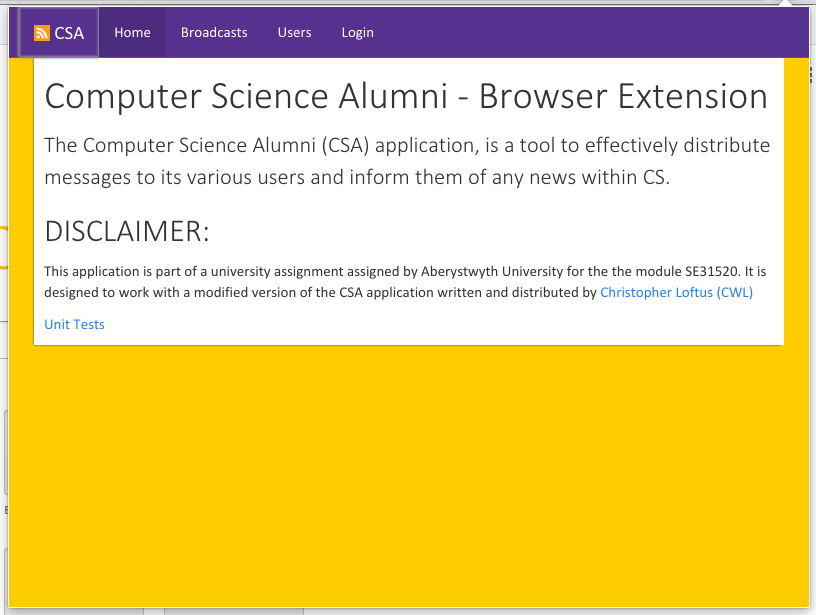
\includegraphics[width=0.7\textwidth]{homepage}
\caption{The screenshot above is the landing screen for the browser extension.}
\end{figure}

\newpage
From the home page the user can navigate to the 'Broadcasts' tab, in the figure captioned there is no broadcasts available to the user so they are show a message that says that there is no broadcasts.\\

\begin{figure}[H]
\centering
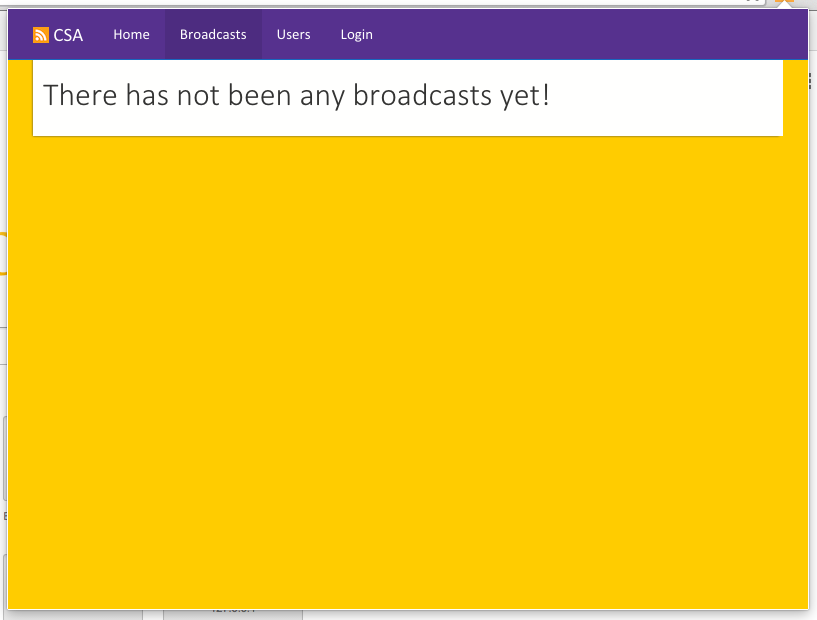
\includegraphics[width=0.7\textwidth]{bcpage}
\caption{Above we see the broadcasts screen with no broadcasts available.}
\end{figure}

Again below we see the 'Broadcasts' tab this time we see how the page appears when there is broadcasts.

\begin{figure}[H]
\centering
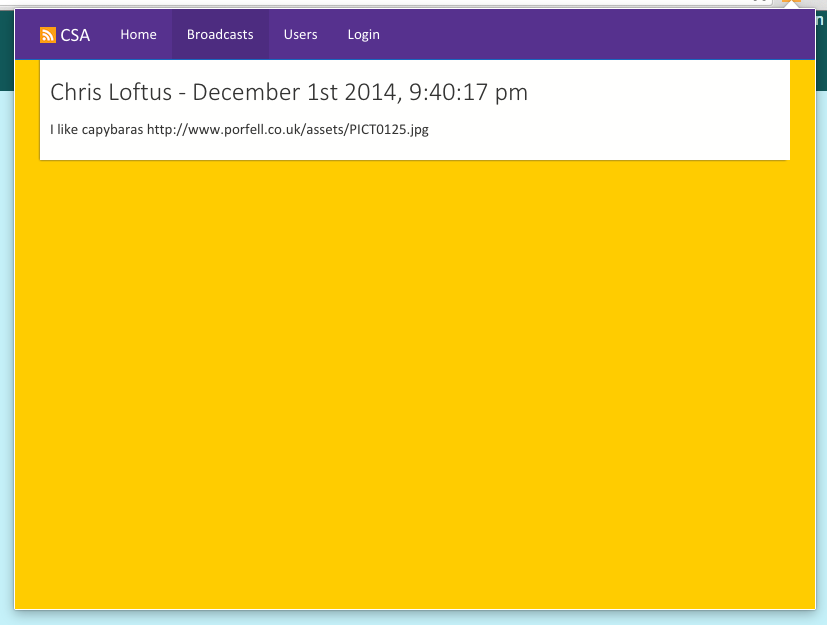
\includegraphics[width=0.7\textwidth]{populatebcpage}
\caption{This is what the populated broadcast screen looks like.}
\end{figure}

This is the 'users' tab of the browser extension here the user can view a specific users details and edit there information if it is deemed appropriate.

\begin{figure}[H]
\centering
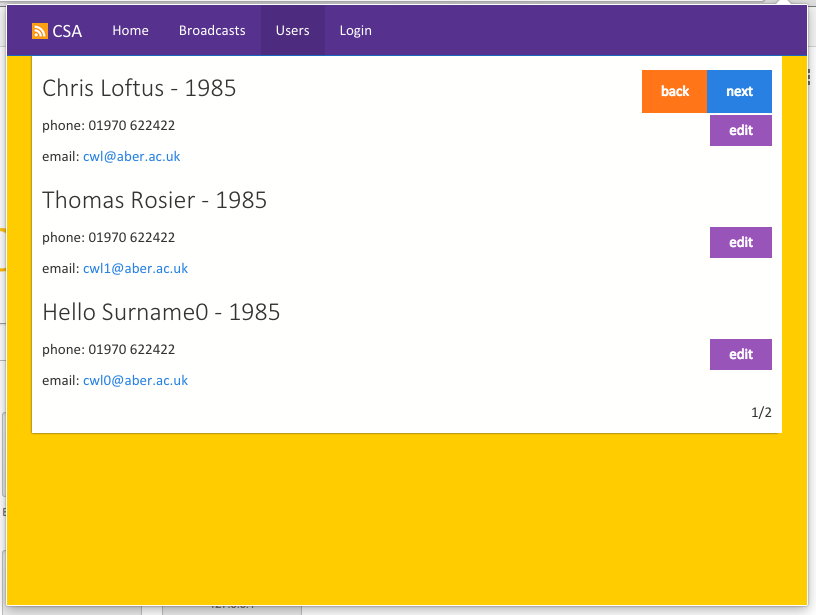
\includegraphics[width=0.7\textwidth]{userpage}
\caption{Here we have a screenshot of the user's screen.}
\end{figure}

When the edit button has pressed on the a specific user it shows this modal window that allows the user to edit the details that are kept on the current user they are editing.

\begin{figure}[H]
\centering
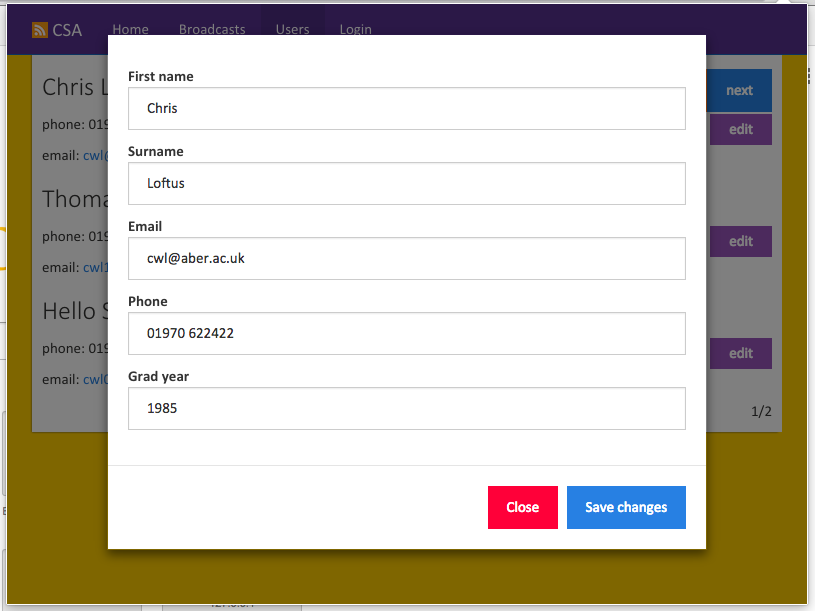
\includegraphics[width=0.7\textwidth]{modalpage}
\caption{Above we have a screenshot showing the modal window we used to edit the user information.}
\end{figure}

\newpage
The 'Login' tab is where the user enters there login credentials that will be used to authenticate the user against the CS-Alumni application.

\begin{figure}[H]
\centering
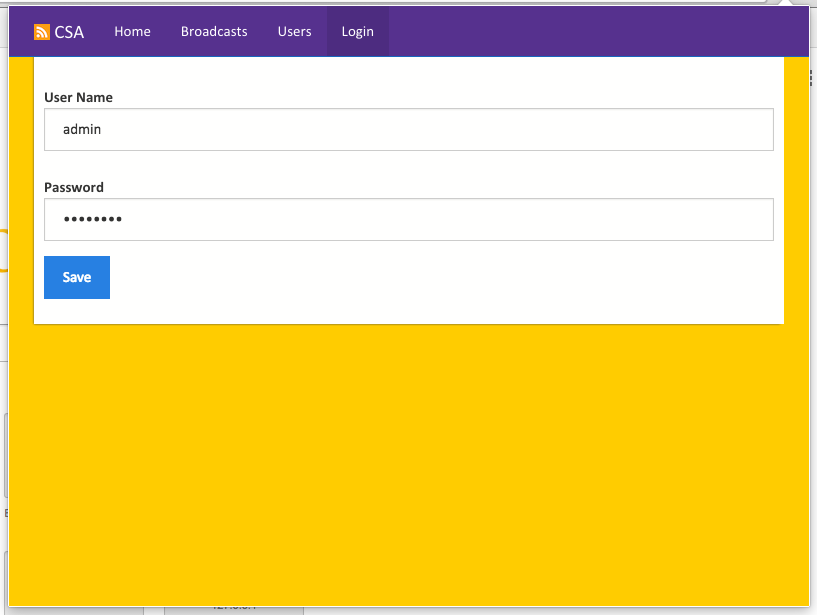
\includegraphics[width=0.7\textwidth]{loginpage}
\caption{This is a screenshot of the login screen.}
\end{figure}

In the screenshot below i have created a new broadcast within the CS-Alumni application to to showcase the notification features within the browser extension.\\
\\
Note: The destination list differs from the standard CSA application. They have been modified to remove the networks that do not work along with adding in the functionality to target the browser extension specifically.\\

\begin{figure}[H]
\centering
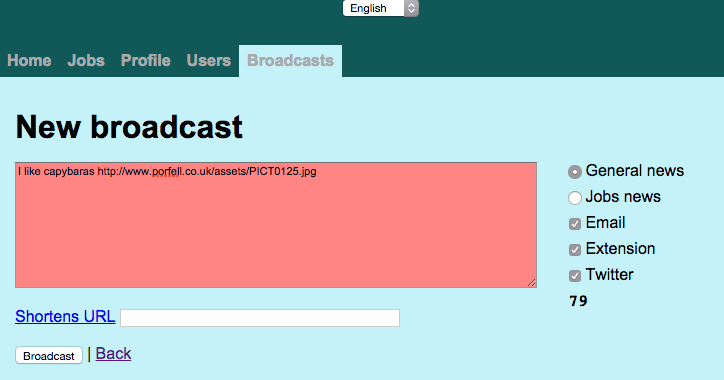
\includegraphics[width=0.75\textwidth]{createbc}
\caption{Creating a broadcast within the CSA application.}
\end{figure}

\newpage
Confirmation of the broadcast being created with the parameters that I gave on the previous screenshot is pictured in the screenshot that has been included below.\\
\\
You can see in the list of feeds that it includes the feed named 'Extension' which signifies that we want to alert users that are using the browser extension.

\begin{figure}[H]
\centering
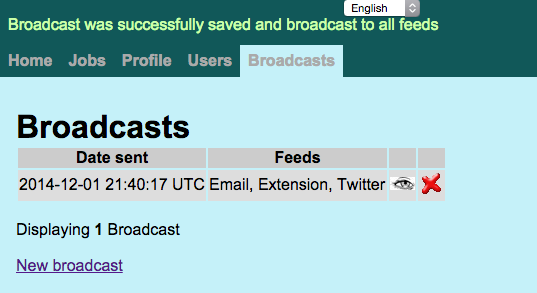
\includegraphics[width=0.75\textwidth]{confbc}
\caption{Here is the confirmation that a new broadcast has been created.}
\end{figure}

Here is shown a Chrome Notification for the broadcast that we just created, this notification will only be shown once when it has been created then is stored and will not be shown again to the user which will prevent them from being annoyed by repeated notifications telling them the same information over and over.

\begin{figure}[H]
\centering

\includegraphics[width=0.5\textwidth]{chromenotification}
\caption{Here is a Chrome notification showing the latest broadcast.}
\end{figure}

Due to the nature of how the browser Opera is designed it users the same core frameworks as Chrome thus allowing it to use the same browser extensions without any modifications the screenshot below shows the same broadcast that we created earlier also being displayed within Opera's notification system.

\begin{figure}[H]
\centering

\includegraphics[width=0.5\textwidth]{operanotification}
\caption{Same again but for Opera this time just to show multi platform support.}
\end{figure}

\newpage
Just to confirm that this is a real broadcast and has not broken any of the other functionality within the CS-Alumni application this is a screenshot of the broadcast on the Twitter website.

\begin{figure}[H]
\centering
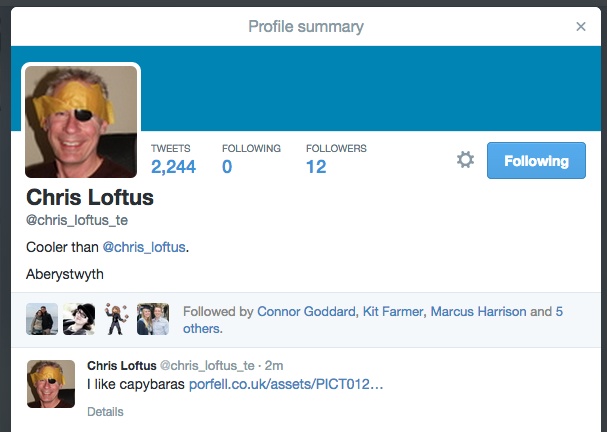
\includegraphics[width=0.8\textwidth]{twitterbc}
\caption{Proof that the broadcasts still get sent to Twitter.}
\end{figure}


\subsection{CS-Alumni Rails Application}

\subsubsection{New Additions}

\paragraph{New Database View}

\paragraph{New RESTful interface}

\subsubsection{Modifications}

\paragraph{Changes to Seeds}

\paragraph{Changes to Broadcasts}

\paragraph{Changes to Security}

\paragraph{Changes to REST implementation}

\paragraph{Changes to Users}

\subsection{Communication Between Applications}

\subsubsection{RESTful Web Interfaces}

\subsubsection{Data Flow Diagrams}


%-- Application Testing.
\newpage
\section{Application Testing}

\subsection{QUnit Tests}

\iffalse
 _________    ________      ________      ________     
|\___   ___\ |\   __  \    |\   ___ \    |\   __  \    
\|___ \  \_| \ \  \|\  \   \ \  \_|\ \   \ \  \|\  \   
     \ \  \   \ \  \\\  \   \ \  \ \\ \   \ \  \\\  \  
      \ \  \   \ \  \\\  \   \ \  \_\\ \   \ \  \\\  \ 
       \ \__\   \ \_______\   \ \_______\   \ \_______\
        \|__|    \|_______|    \|_______|    \|_______|                                               
\fi   

\begin{figure}[H]
\centering
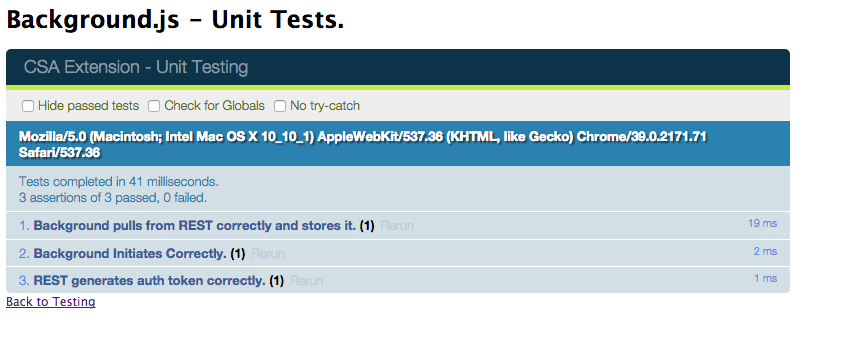
\includegraphics[width=\textwidth]{backgroundqunit}
\caption{This is the unit tests for the background.js module for the browser extension.}
\end{figure}

\begin{figure}[H]
\centering
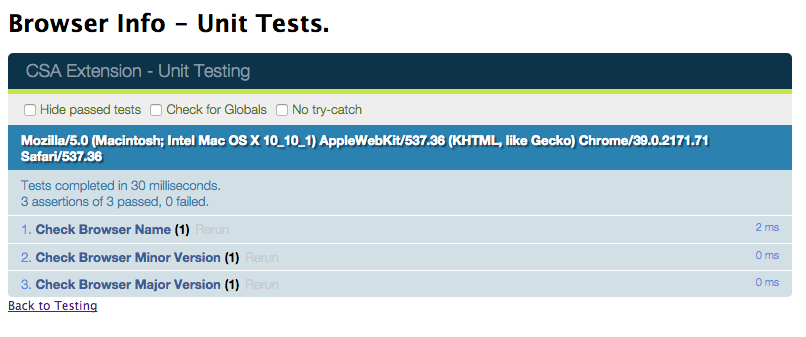
\includegraphics[width=\textwidth]{biqunit}
\caption{This images shows the browserinfo.js module completing its tests successfully.}
\end{figure}

\begin{figure}[H]
\centering
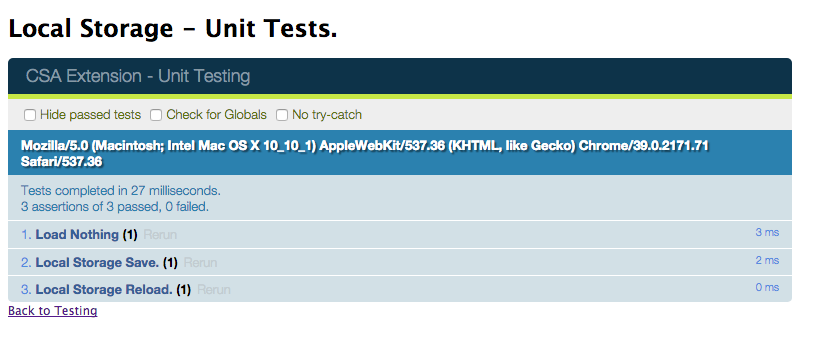
\includegraphics[width=\textwidth]{lsqunit}
\caption{This shows the LocalStorage.js module passing all its unit tests.}
\end{figure}

\begin{figure}[H]
\centering
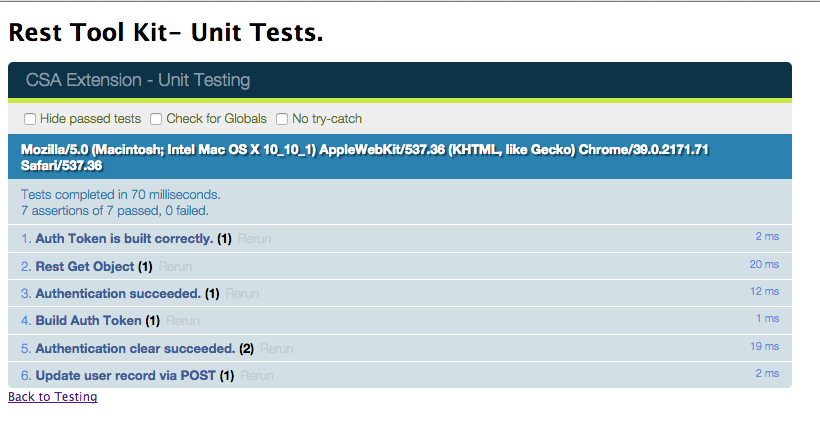
\includegraphics[width=\textwidth]{restqunit}
\caption{Above we see the RestToolKit.js module successfully completing all its unit tests.}
\end{figure}

\begin{figure}[H]
\centering
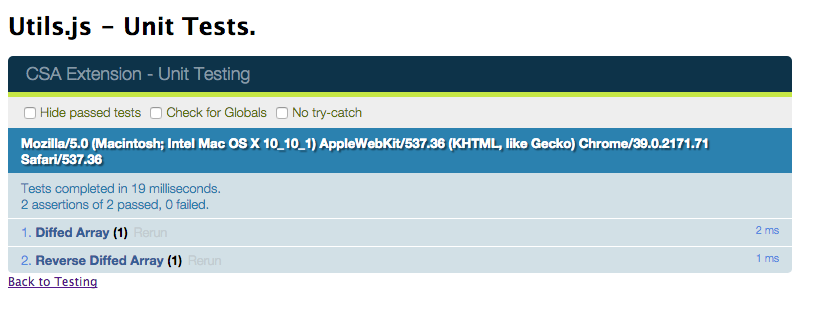
\includegraphics[width=\textwidth]{utilsqunit}
\caption{Included above we see the Utils.js module efficiently complete all of its unit tests.}
\end{figure}

%-- Technologies.
\newpage
\section*{Technologies}

\subsection{CS-Alumni Chrome Browser Extension}

\subsubsection{Javascript}

\subsubsection{Chrome Extensions API}

\subsubsection{Bootstrap}

\subsubsection{jQuery}

\subsubsection{Moment.js}

\subsubsection{Alertify.js}

\subsubsection{Qunit}

\subsection{CS-Alumni Rails Application}

\subsubsection{Ruby}

\subsubsection{Ruby on rails}

\subsubsection{Qunit}

\subsection{Communication Between Applications}

\subsubsection{RESTful Interfaces}

\subsubsection{CORS}

\subsubsection{Basic Authentication}

%-- Evaluation.
\newpage
\section{Evaluation}

\iffalse
 _________    ________      ________      ________     
|\___   ___\ |\   __  \    |\   ___ \    |\   __  \    
\|___ \  \_| \ \  \|\  \   \ \  \_|\ \   \ \  \|\  \   
     \ \  \   \ \  \\\  \   \ \  \ \\ \   \ \  \\\  \  
      \ \  \   \ \  \\\  \   \ \  \_\\ \   \ \  \\\  \ 
       \ \__\   \ \_______\   \ \_______\   \ \_______\
        \|__|    \|_______|    \|_______|    \|_______|                                               
\fi   

\newpage
\section{Something Extra}
%-- Talk about pebble app here.
\begin{figure}[H]
\centering
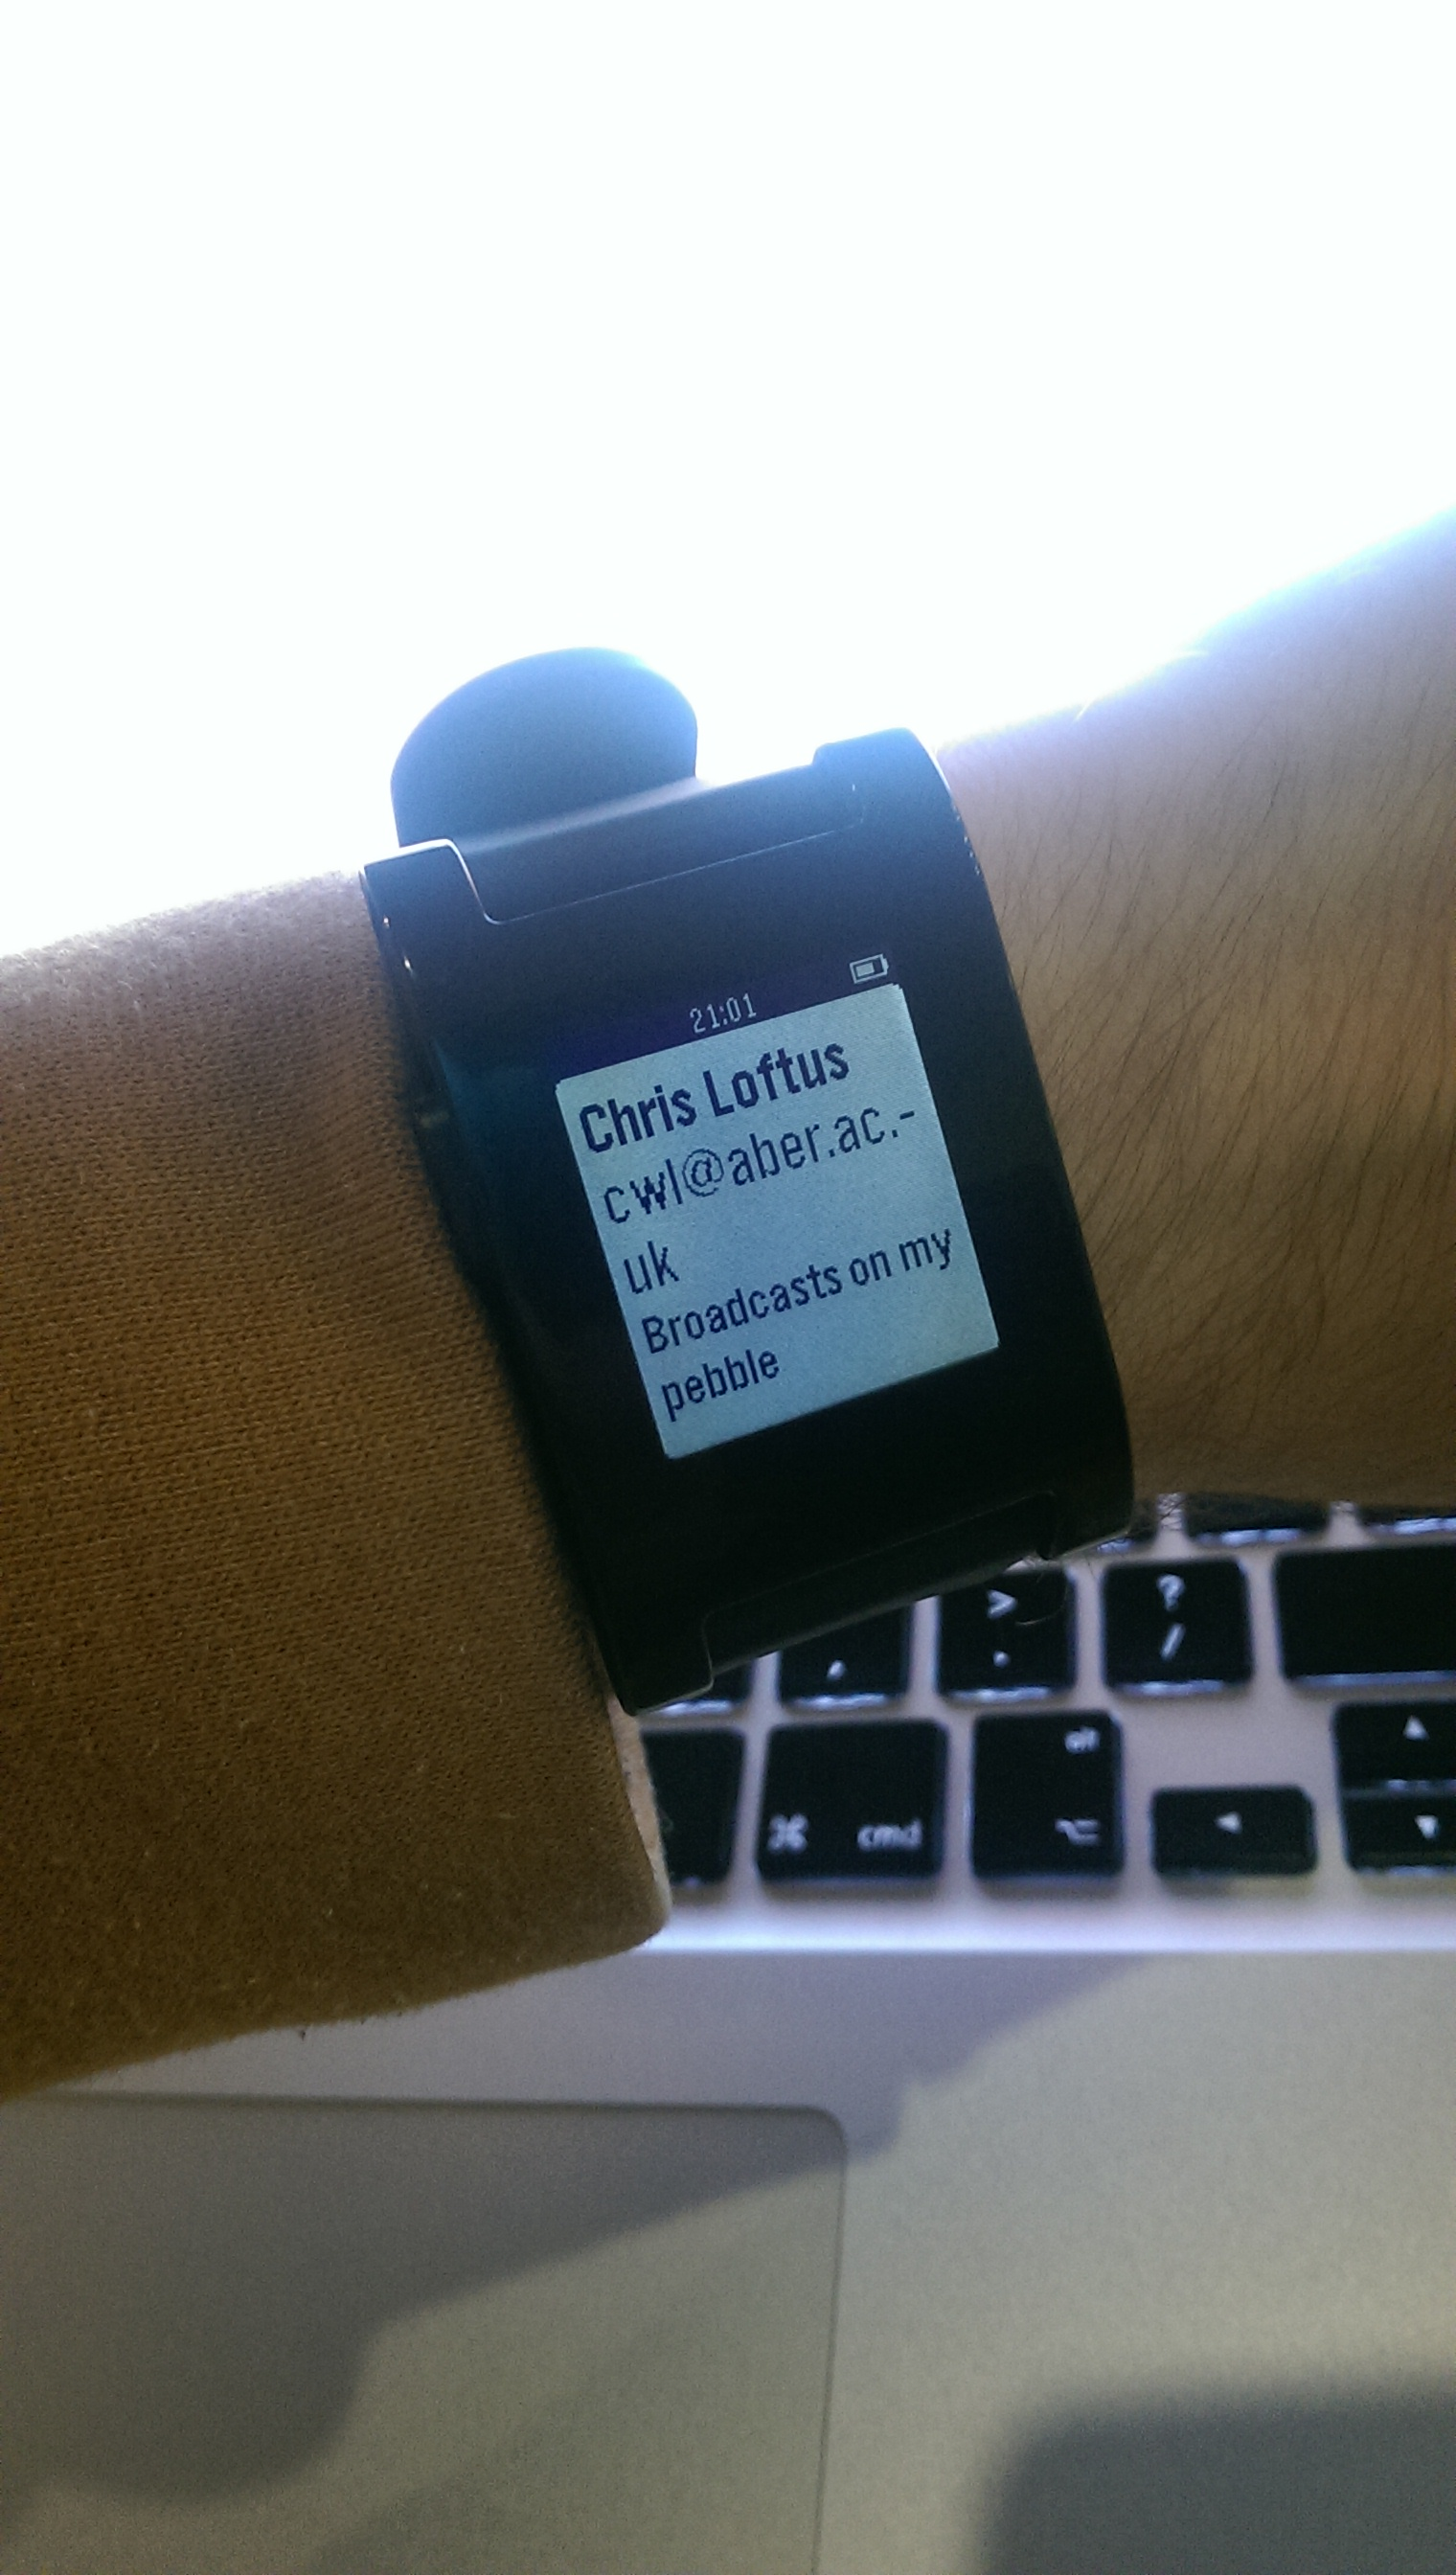
\includegraphics[width=0.5\textwidth]{pebble}
\caption{Above is a image of the Pebble smartwatch running the CSA application.}
\end{figure}

\begin{figure}[H]
\centering
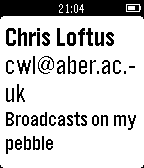
\includegraphics[width=0.25\textwidth]{pebblesh}
\caption{This is a screenshot taken from the Pebble smartwatch.}
\end{figure}

\newpage
%-- Attributions.
\section*{Attributions}

\newpage
\printbibliography

\end{document}